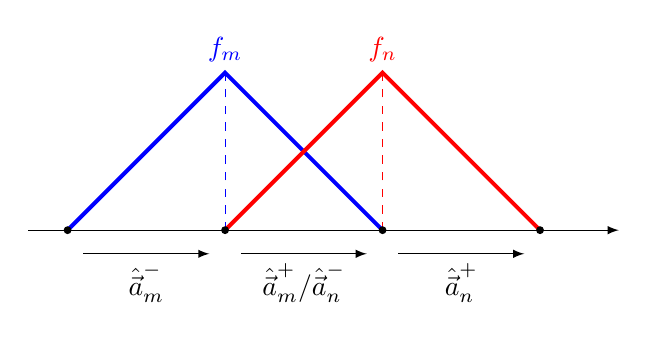
\begin{tikzpicture}[> = latex]
	\draw[->] (-0.5, 0) -- (7, 0);	
	
	\draw[blue, line width=0.5mm] (0, 0) -- (2, 2) node[above] {$f_m$} -- (4, 0);
	\draw[red, line width=0.5mm] (2, 0) -- (4, 2) node[above] {$f_n$} -- (6, 0);
	\draw[blue, dashed] (2, 0) -- (2, 2);
	\draw[red, dashed] (4, 0) -- (4, 2);
	\node[fill = black, circle, inner sep=0pt, minimum size = 1mm] at (0, 0) {};
	\node[fill = black, circle, inner sep=0pt, minimum size = 1mm] at (2, 0) {};
	\node[fill = black, circle, inner sep=0pt, minimum size = 1mm] at (4, 0) {};
	\node[fill = black, circle, inner sep=0pt, minimum size = 1mm] at (6, 0) {};
	
	\draw[->] (0.2, -0.3) -- node[below] {$\hat{\vec{a}}_m^{-}$} (1.8, -0.3);
	\draw[->] (2.2, -0.3) -- node[below] {$\hat{\vec{a}}_m^{+}$/$\hat{\vec{a}}_n^{-}$} (3.8, -0.3);
	\draw[->] (4.2, -0.3) -- node[below] {$\hat{\vec{a}}_n^{+}$} (5.8, -0.3);
\end{tikzpicture}